\documentclass[slidestop,usenames,dvipsnames]{beamer}
\usepackage[utf8]{inputenc}
\usepackage[T1]{fontenc}
\usepackage{graphicx}
\usepackage[yyyymmdd]{datetime}
\renewcommand{\dateseparator}{-}

\title{Network Cascades}
\subtitle{The Grim Truth Revealed}
\author{Marco Brack \and Carsten Hartenfels}

\beamertemplatenavigationsymbolsempty
\usetheme{Boadilla}
\usecolortheme{whale}
\setbeamertemplate{itemize items}[default]
\setbeamertemplate{enumerate items}[default]
\defbeamertemplate*{footline}{my infolines theme} {
    \leavevmode
    \hbox{
    \begin{beamercolorbox}[wd=.333333\paperwidth,ht=2.25ex,dp=1ex,center]{author in head/foot}
        \usebeamerfont{author in head/foot}Marco Brack, Carsten Hartenfels
    \end{beamercolorbox}
    \begin{beamercolorbox}[wd=.333333\paperwidth,ht=2.25ex,dp=1ex,center]{title in head/foot}
        \usebeamerfont{title in head/foot}Network Cascades
    \end{beamercolorbox}
    \begin{beamercolorbox}[wd=.309\paperwidth,ht=2.25ex,dp=1ex,center]{date in head/foot}
        \usebeamerfont{date in head/foot}\insertshortdate{}\hspace*{2em}
        \insertframenumber{} / \inserttotalframenumber\hspace*{2ex}
    \end{beamercolorbox}}
    \vskip0pt
}

\newcommand{\fitem}{\pause\vfill\item}
\newcommand{\gitem}{\vfill\item}

\begin{document}

\begin{frame}
    \titlepage
\end{frame}


%%%%%%%%%%%%%%%%%%%%%%%%%%%%%%%%%%%%%%%%%%%%%%%%


\begin{frame}
    \frametitle{Content}
    \begin{itemize}
        \gitem Motivation
        \gitem Model of Doom
        \gitem Another Model of Doom
        \gitem Doomsday Scenarios
    \end{itemize}
    \vfill
\end{frame}


\begin{frame}
    \frametitle{Motivation}
    \begin{itemize}
        \fitem Twilight
        \fitem WhatsApp
        \fitem Political Coups
        \fitem Job Interviews
    \end{itemize}
    \vfill
\end{frame}

\begin{frame}
    \frametitle{The Cause Revealed}
    \vfill
    \begin{center}
        \pause {\Huge \underline{Network Cascades}}\\
        \vspace{20pt}
        \pause {\footnotesize (Maybe)}\\
        \vspace{20pt}
        \pause {\footnotesize (It's a Nice Model Anyway)}
    \end{center}
    \vfill
\end{frame}

% too much clutter
\begin{frame}
    \frametitle{Model of Doom}
    \begin{itemize}
        \gitem Nodes
    \end{itemize}
    \vfill
    \includegraphics[width=\textwidth]{img/model1}
    \vfill
\end{frame}

\begin{frame}
    \frametitle{Model of Doom}
    \begin{itemize}
        \gitem Observe $k$ Neighbors
    \end{itemize}
    \vfill
    \includegraphics[width=\textwidth]{img/model2}
    \vfill
\end{frame}

\begin{frame}
    \frametitle{Model of Doom}
    \begin{itemize}
        \gitem State $\in \lbrace 0, 1 \rbrace$
    \end{itemize}
    \vfill
    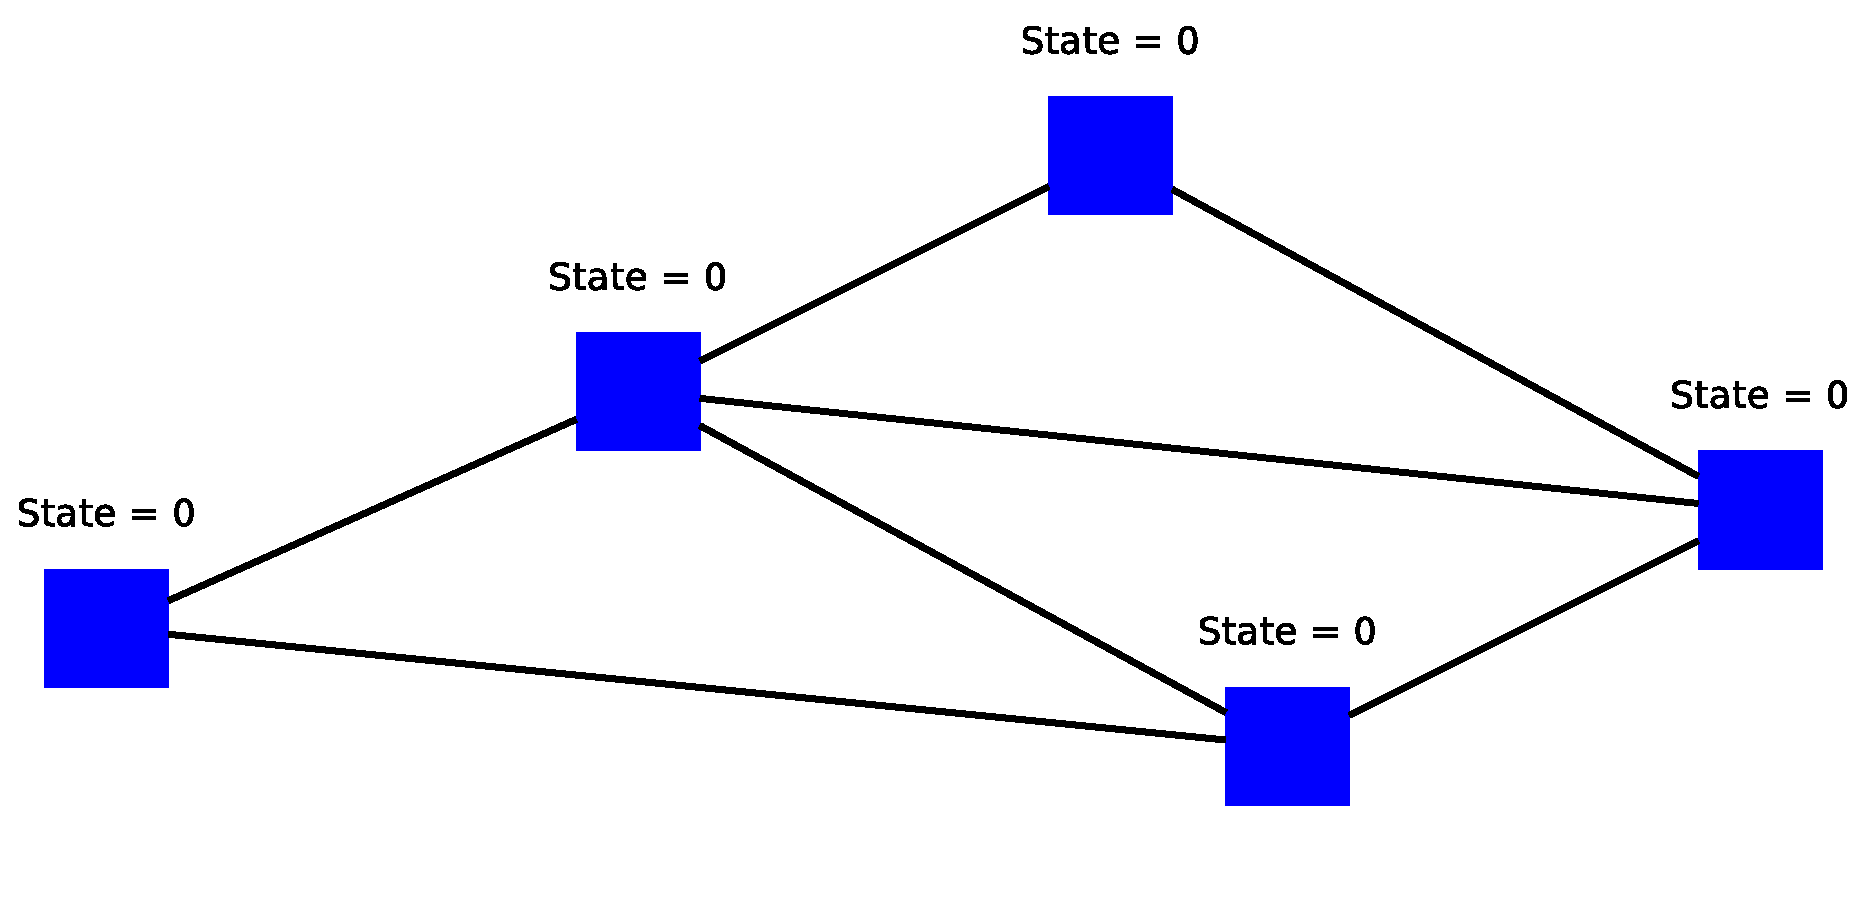
\includegraphics[width=\textwidth]{img/model3}
    \vfill
\end{frame}

\begin{frame}
    \frametitle{Model of Doom}
    \begin{itemize}
        \gitem Threshold $\Phi \in [0, 1]$
    \end{itemize}
    \vfill
    \includegraphics[width=\textwidth]{img/model4}
    \vfill
\end{frame}

\begin{frame}
    \frametitle{Model of Doom}
    \begin{itemize}
        \gitem Random Impulse Happens
    \end{itemize}
    \vfill
    \includegraphics[width=\textwidth]{img/model5}
    \vfill
\end{frame}

\begin{frame}
    \frametitle{Model of Doom}
    \begin{itemize}
        \gitem Nodes Check in Random Intervals
    \end{itemize}
    \vfill
    \includegraphics[width=\textwidth]{img/model6}
    \vfill
\end{frame}

\begin{frame}
    \frametitle{Model of Doom}
    \begin{itemize}
        \gitem Stuff Happens
    \end{itemize}
    \vfill
    \includegraphics[width=\textwidth]{img/model7}
    \vfill
\end{frame}

\begin{frame}
    \frametitle{Model of Doom}
    \begin{itemize}
        \gitem Things Occur
    \end{itemize}
    \vfill
    \includegraphics[width=\textwidth]{img/model8}
    \vfill
\end{frame}

\begin{frame}
    \frametitle{Model of Doom}
    \begin{itemize}
        \gitem Coup Successful
    \end{itemize}
    \vfill
    \includegraphics[width=\textwidth]{img/model9}
    \vfill
\end{frame}


\begin{frame}
    \frametitle{Limitations}
    \begin{itemize}
        \fitem No Personal Knowledge
        \fitem No Global Adoption Rate
        \fitem No Relationship Strength
        \fitem One-Way Threshold
    \end{itemize}
    \vfill
\end{frame}

\begin{frame}
    \frametitle{An Alternative: Cascading Models}
    \begin{itemize}
        \fitem Activation Success Propabilities for Edges
        \fitem Nodes Try Activating Neighbors After Being Activated
        \fitem Succeeds With Specified Propability
        \fitem May Incorporate Both Nodes and History of Activation Attempts
    \end{itemize}
    \vfill
\end{frame}

\begin{frame}
    \frametitle{(Ab)using Information Cascades}
    \begin{itemize}
        \fitem Be Greedy Capitalist Pig
        \fitem Want to Promote New Product
        \fitem Convincing Individuals is Hard/Expensive
        \fitem Convincing at Least Some Individuals in a Group is More Cost-Effective
        \fitem Target Group in Hopes of Starting a Cascade
        \fitem Stoopid Sheeple Follow the Herd
        \fitem ???
        \fitem Profit
    \end{itemize}
    \vfill
    Source: \cite{eftekhar2013information}
\end{frame}


%%%%%%%%%%%%%%%%%%%%%%%%%%%%%%%%%%%%%%%%%%%%%%%%


\begin{frame}
    \vfill
    \begin{center}
        {\Huge Thank You All For Listening}\
    \end{center}
\end{frame}

\bibliographystyle{alpha}
\bibliography{../bibliography/bibliography}

\end{document}
